% !TEX root = ejb-web.tex
%!TEX encoding = UTF-8 Unicode
\ifx\setbeamertemplate\undefined
\documentclass[handout]{beamer}
\fi
\graphicspath{{../images/}}
\usepackage{amsmath}
\usepackage{xifthen}

\usepackage{mathtools}
\mathtoolsset{showonlyrefs}
\usepackage{mathrsfs}

\usepackage[multidot]{grffile}

\usepackage{xspace}
\usepackage{upgreek}
\newcommand\xsb{$\upchi$SB\xspace}
\newlength{\imagecolumnwidth}

\usepackage[absolute,overlay]{textpos}

\usepackage{slashed}
\newcommand\dslash{\slashed{\partial}}

\usepackage{bbold}
\newcommand\one{\mathbb{1}}

\usepackage{multirow}

\newcommand\bs\boldsymbol

\newcommand \Sx[1] {S_{\textnormal{#1}}}
\newcommand \Sg[2] {\mathrm{#1}(#2)}
\newcommand \SU[1] {\Sg{SU}{#1}}
\newcommand \SO[1] {\Sg{SO}{#1}}
\newcommand \Sp[1] {\Sg{Sp}{#1}}
\newcommand \Uone {\Sg{U}{1}}

\newcommand\pb{\overline{\psi}}
\newcommand \bigL {\mathscr{L}}
\newcommand \lag[1] {\bigL_{\mathrm{#1}}}

\newcommand\sptn{Sp($2N$)\xspace}
\newcommand\dee{\mathrm{d}}
\newcommand\eee{\mathcal{E}}
\newcommand\www{\mathcal{W}}
\DeclareMathOperator\tr{tr}
\DeclareMathOperator\real{Re}
\newcommand\Nf{N_{\mathrm{f}}}

%\usepackage{beamerthemesplit} %Activate for custom appearance
\setbeamertemplate{navigation symbols}{}%remove navigation symbols

\usefonttheme[onlymath]{serif}
\usepackage{fontspec,xltxtra,xunicode}
\defaultfontfeatures{Mapping=tex-text}
\setsansfont[Scale=MatchLowercase,Mapping=tex-text]{Futura}
\setbeamerfont{structure}{family=\fontspec{Cosmos BQ}}
\definecolor{swanseablue}{RGB}{36,47,96}
\setbeamercolor{structure}{fg=swanseablue}
 \setbeamertemplate{itemize item}{•}
 \setbeamertemplate{itemize subitem}{--}
 \setbeamercolor{itemize item}{fg=black}
 \setbeamercolor{itemize subitem}{fg=black}

\newcommand\disappear[1]{}
\title{Profiling MPI code to identify bottlenecks}
\author{{\large Ed Bennett}
	\\{\small@QuantumofEd}
	\\\vspace{16pt}
	\hfill
	\parbox{0.22\textwidth}{\centering
\includegraphics[height=36pt]{logos/swansea}\\\small @SwanseaUni}
	\parbox{0.44\textwidth}{\centering
\includegraphics[height=24pt]{logos/scw}\\\small @SuperCompWales}
	\parbox{0.22\textwidth}{\centering
\includegraphics[height=36pt]{logos/sa2c}\\\small @sa2c\_swansea} }
\date{Supercomputing Wales Swansea Symposium, 2018-09-13}

\newcommand\Wider[2][3em]{%
\makebox[\linewidth][c]{%
  \begin{minipage}{\dimexpr\paperwidth-#1\relax}
  \raggedright#2
  \end{minipage}%
  }%
}



\newcommand\FrameText[1]{%
  \begin{textblock*}{0.9\paperwidth}(3pt, 0.99\textheight)
    \raggedright #1\hspace{.5em}
  \end{textblock*}}

\newcommand \sechead[1] {\frame{\vfill\Huge \centering\usebeamerfont{structure}\color{swanseablue}#1\vfill\null}}

\usebackgroundtemplate%
{%
	
\includegraphics[width=\paperwidth,height=\paperheight]{background/bg}%
}
\setbeamertemplate{footline}{
	\vspace{1.0cm}
}


  
\begin{document}

\frame{\titlepage}

\begin{frame}[fragile]{MPI, briefly}
	\begin{itemize}[<+->]
		\item MPI: \textbf{M}essage \textbf{P}assing \textbf{I}nterface
		\item Born in 1991, now at version 3.1
		\item Single Program Multiple Data model
		\begin{itemize}[<+->]
			\item Same program runs multiple times (on one or more nodes)
			\item Communication is explicit
		\end{itemize}
		\item Point-to-point send and receive
		\item \textbf{I}mmediate (non-blocking) versions
		\item Point-to-all (broadcast) operations
		\item Collectives, e.g. reductions (sums, maxima, minima, etc.)
	\end{itemize}
\end{frame}

\begin{frame}[fragile]{Profiling MPI}
	\begin{itemize}[<+->]
		\item Intel MPI provides profiling tools
		\begin{verbatim}source /apps/compilers/intel/2018.3/itac_2018/bin/itacvars.sh
mpirun -trace [my_application]\end{verbatim}
		\item Output can be \emph{large}, so choose a small problem size
		\item Visualise the results with \verb|traceanalyzer|
	\end{itemize}
\end{frame}

\begin{frame}{Summary view}
	\centering
	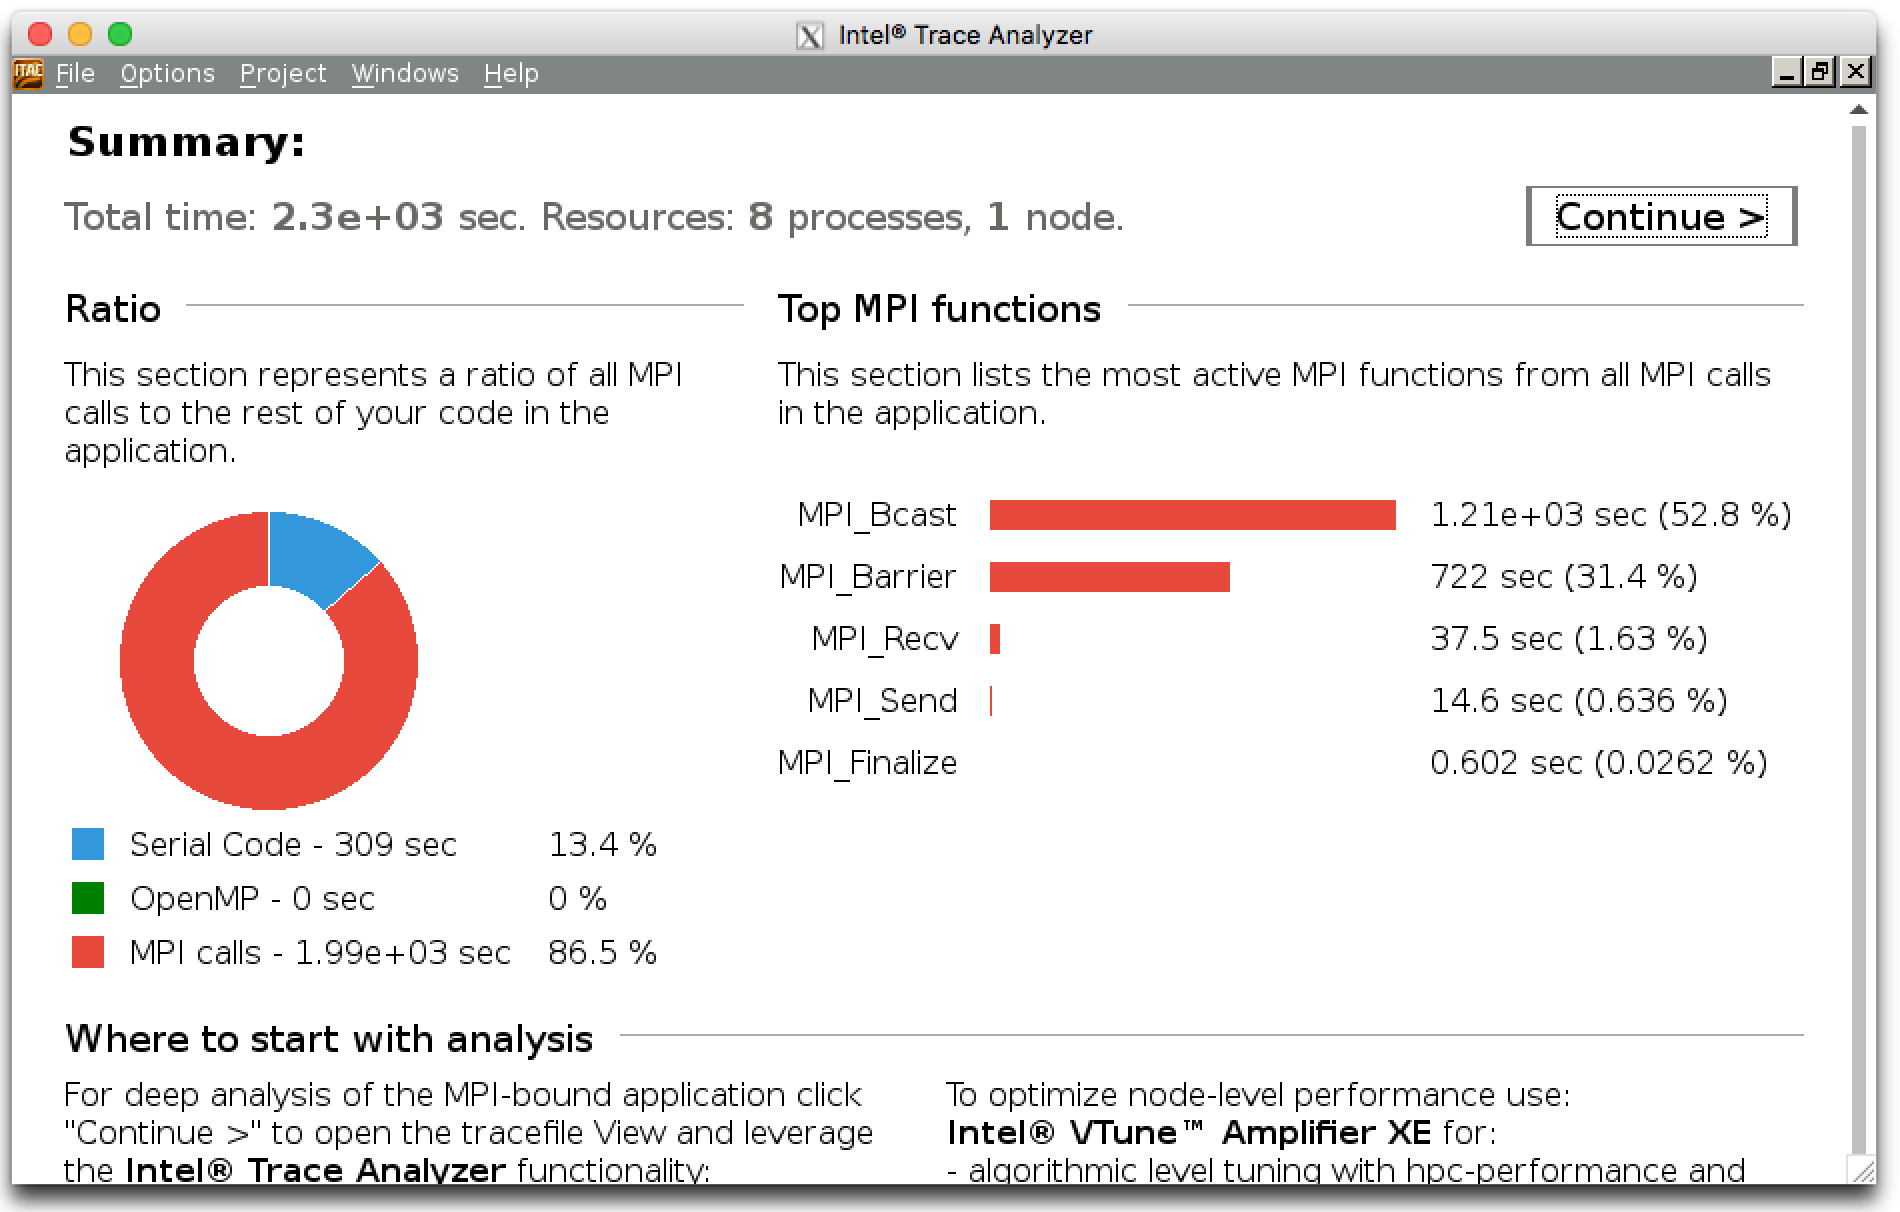
\includegraphics[width=0.8\textwidth]{figs/first-overview}
\end{frame}

\begin{frame}{Whole application timeline}
	\centering
	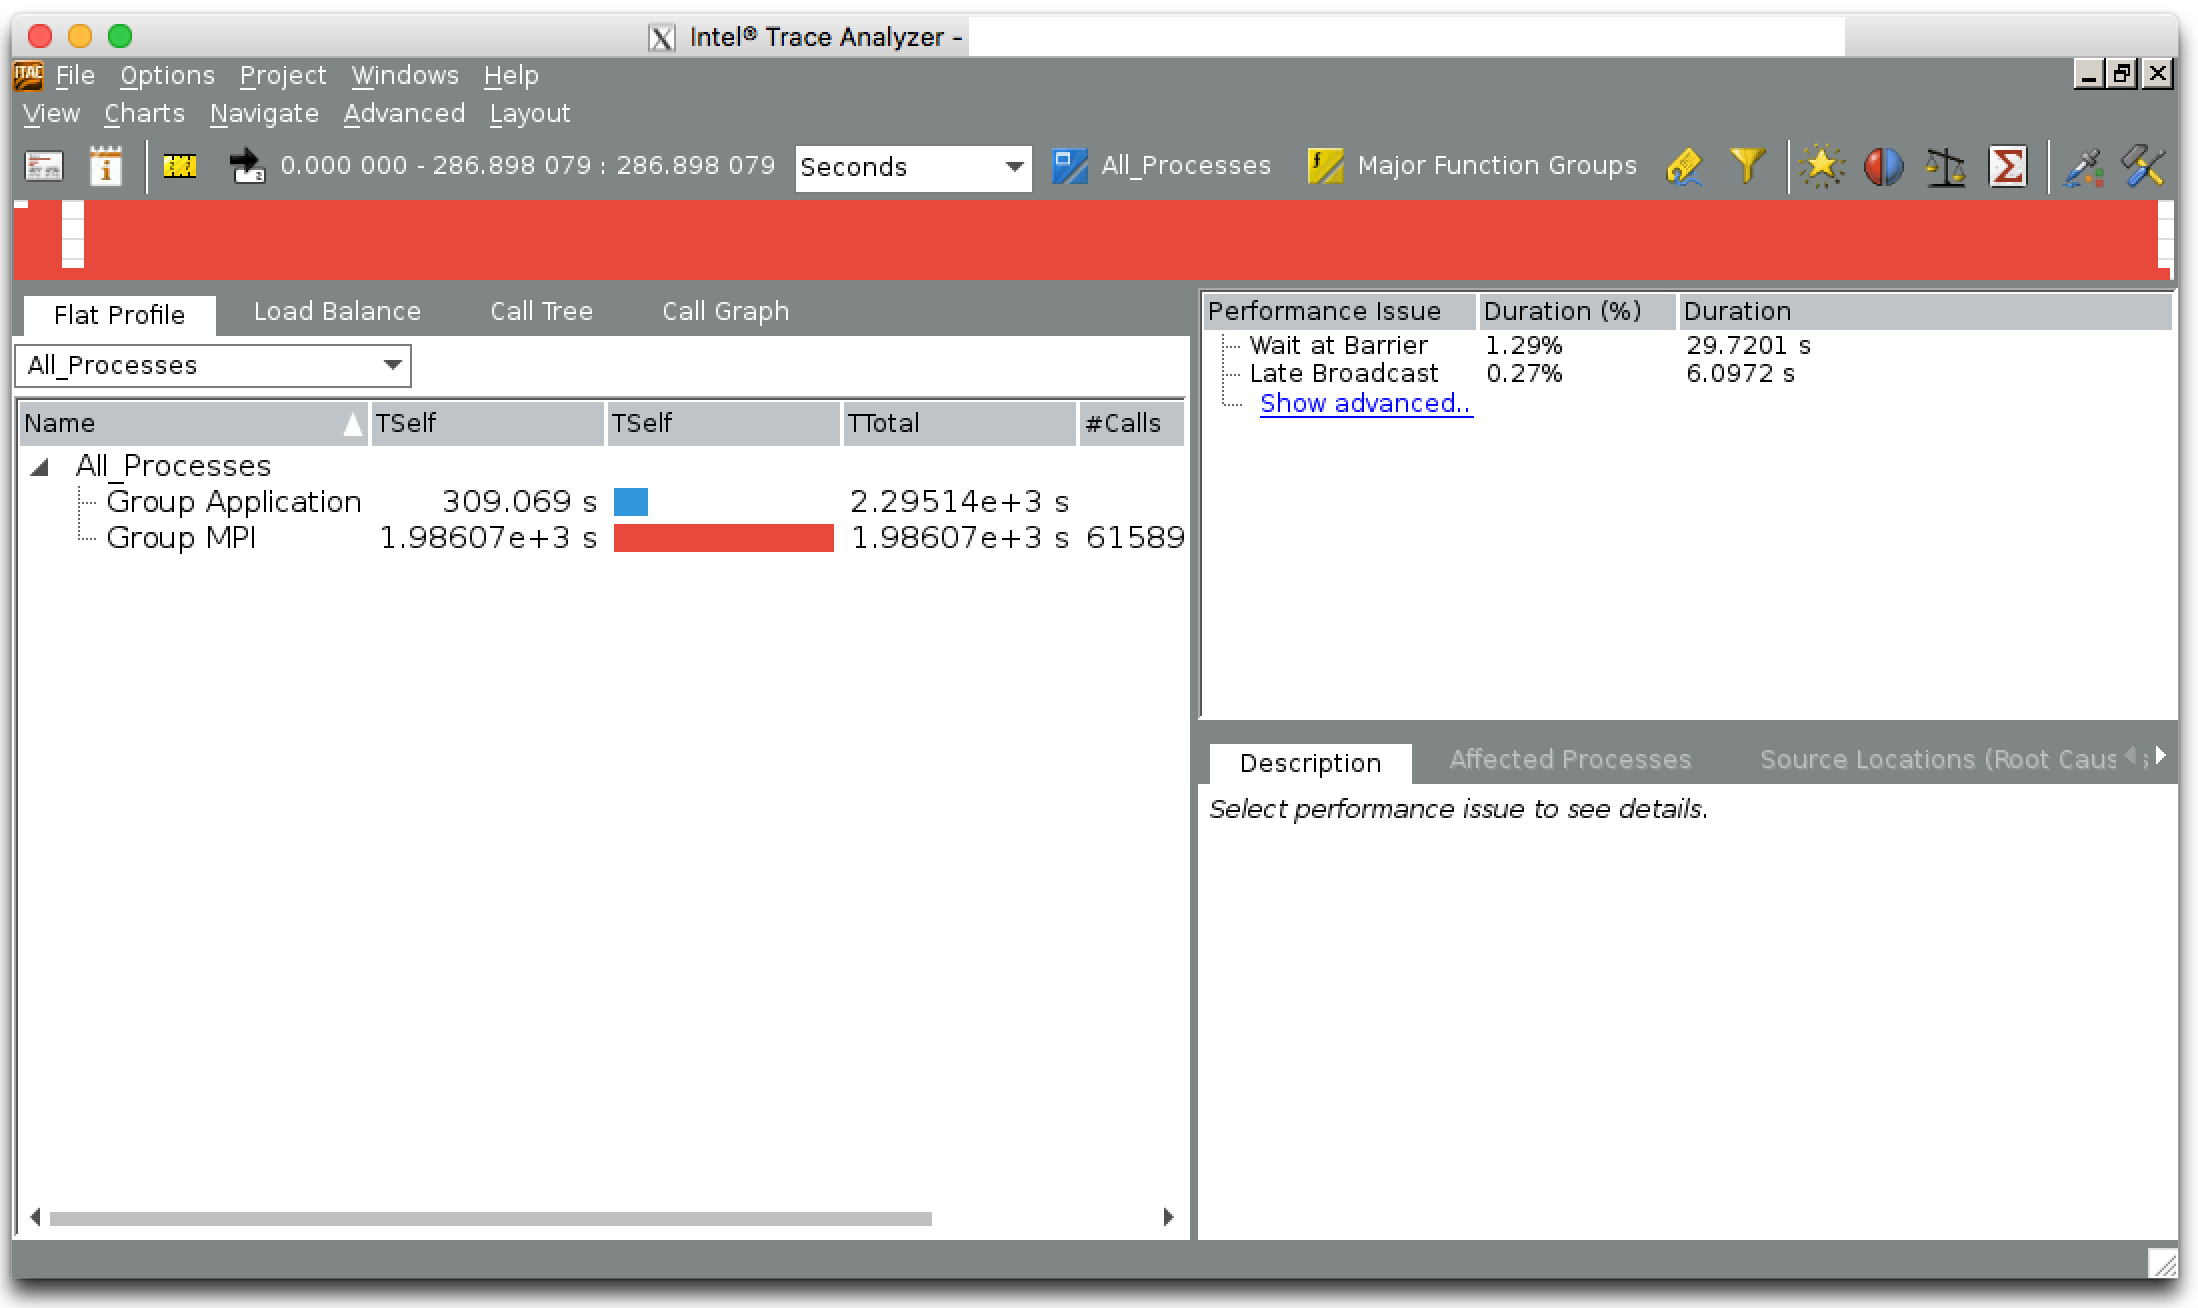
\includegraphics[width=0.8\textwidth]{figs/overview-timeline}
\end{frame}

\begin{frame}{Detailed timeline}
	\centering
	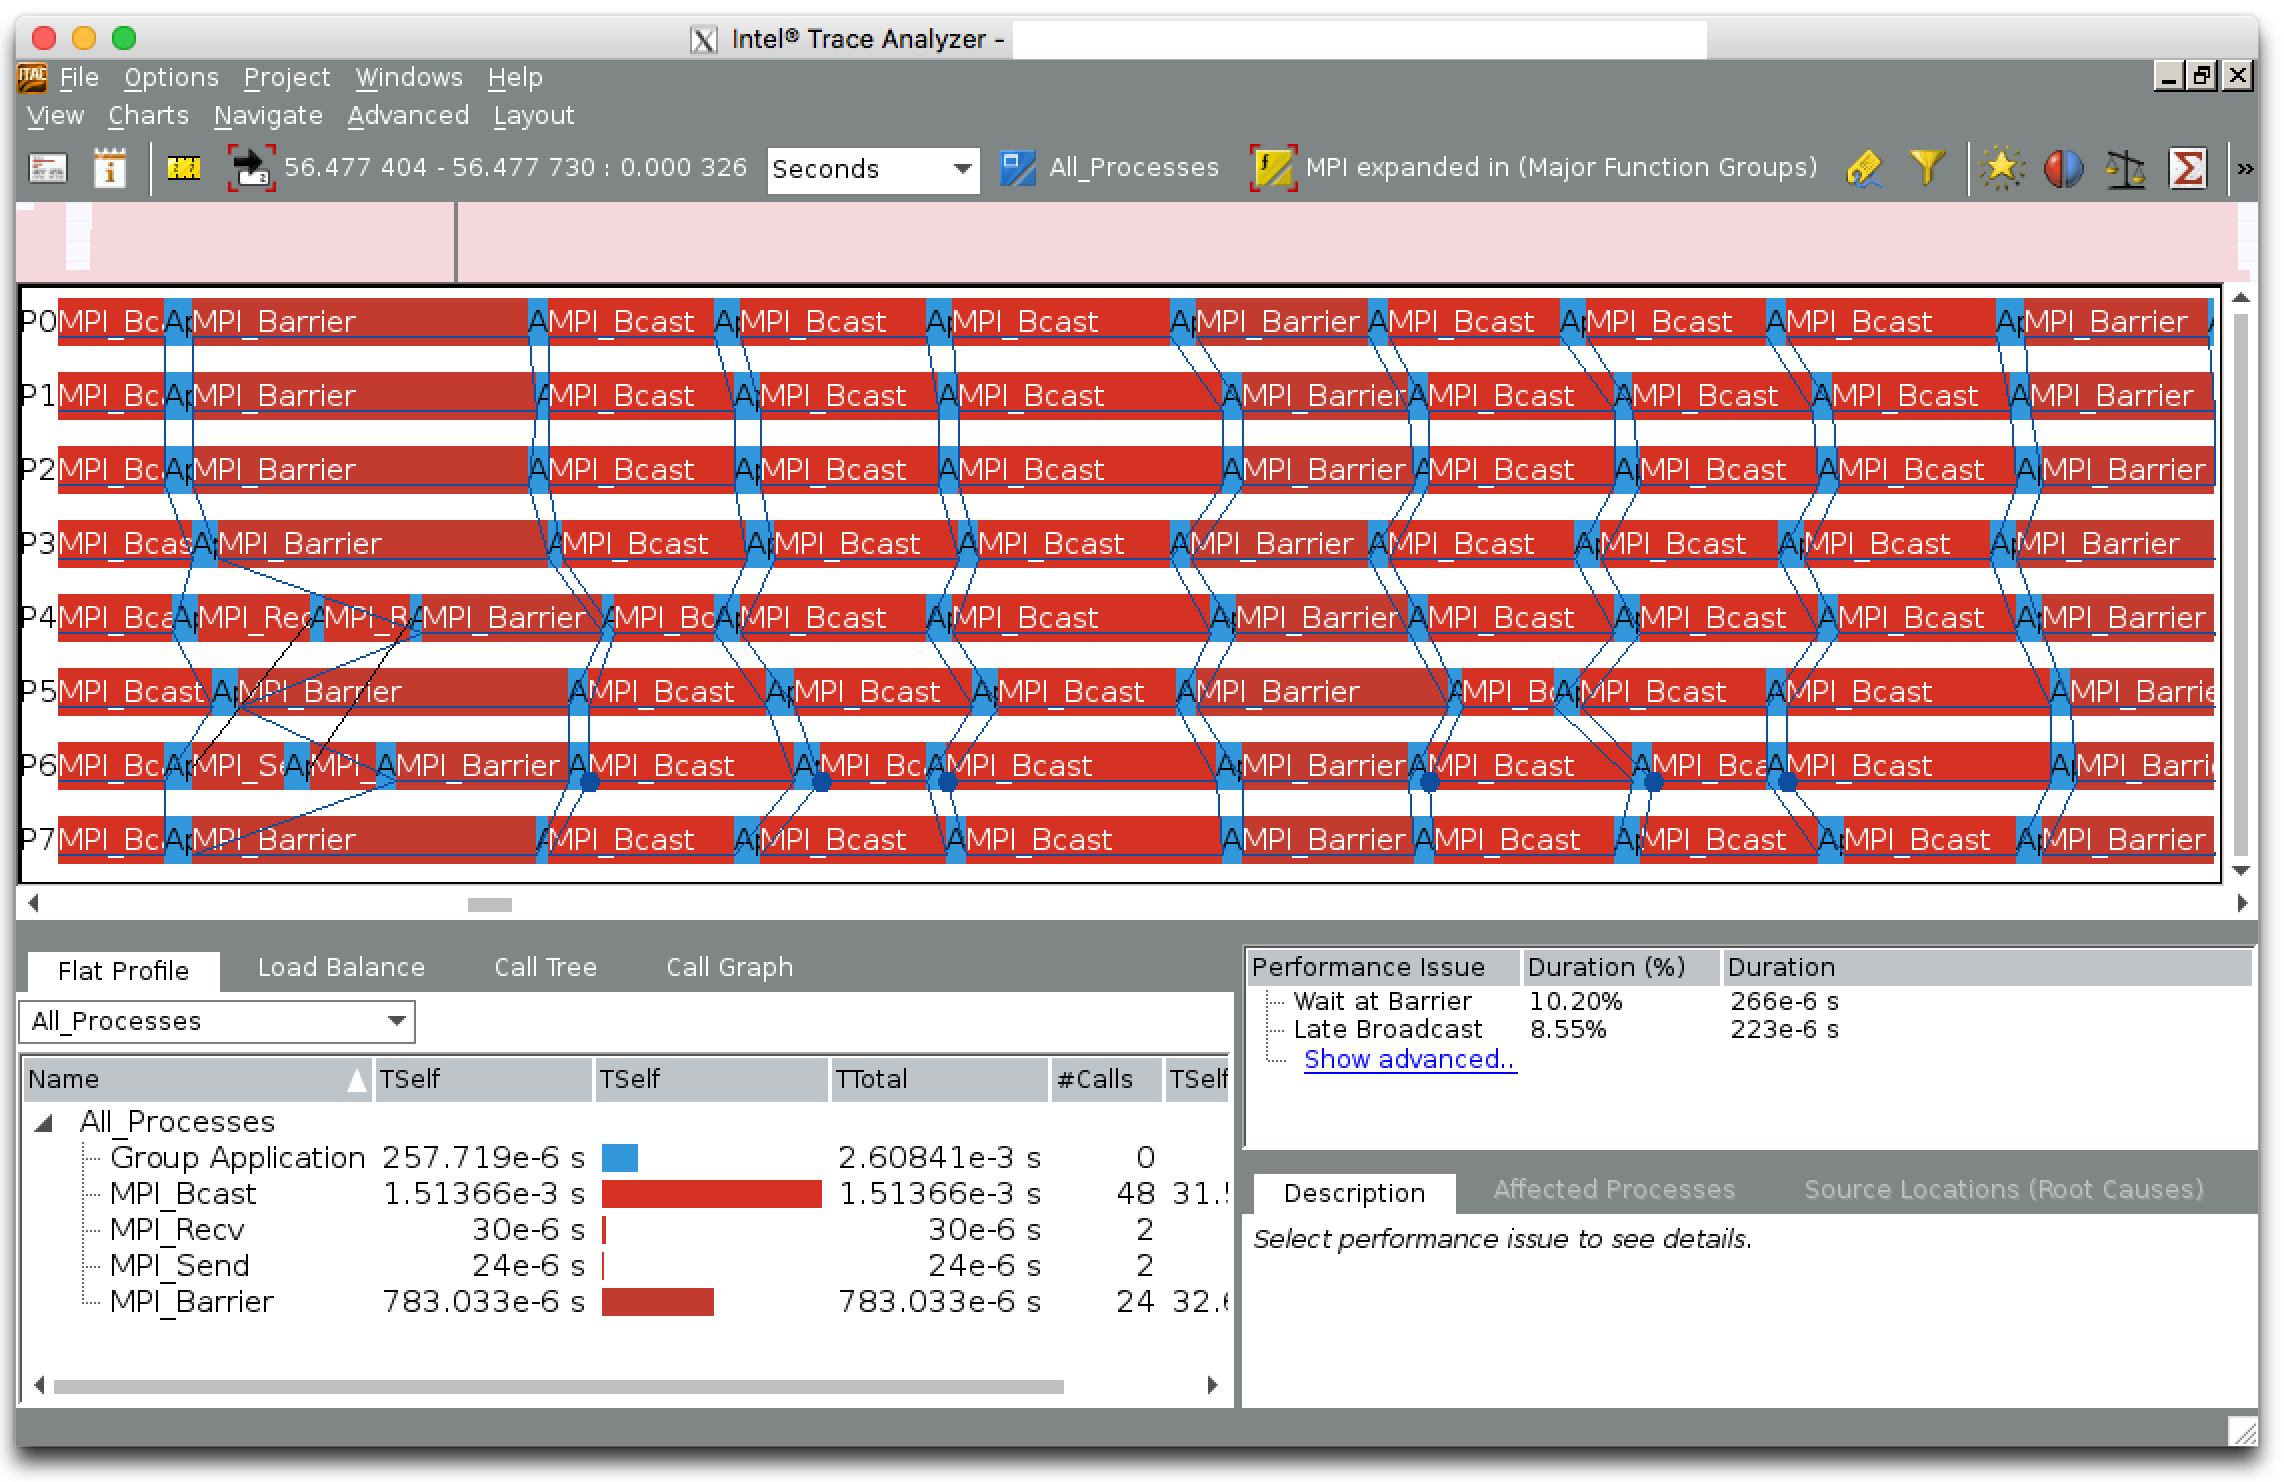
\includegraphics[width=0.78\textwidth]{figs/detailed-timeline}
\end{frame}

\begin{frame}{Message pattern}
	\centering
	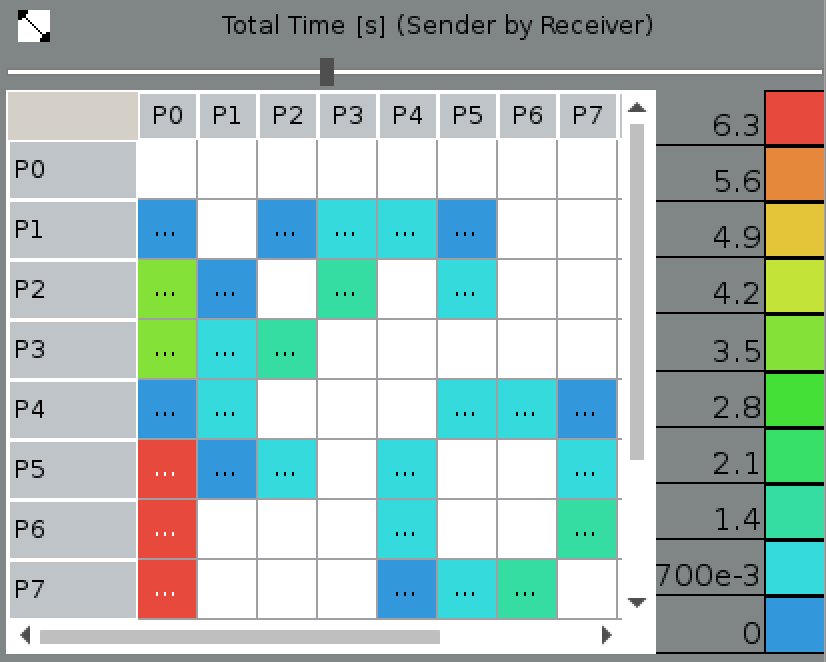
\includegraphics[width=0.6\textwidth]{figs/message-pattern}
\end{frame}

\begin{frame}{Reductions summary}
	\centering
	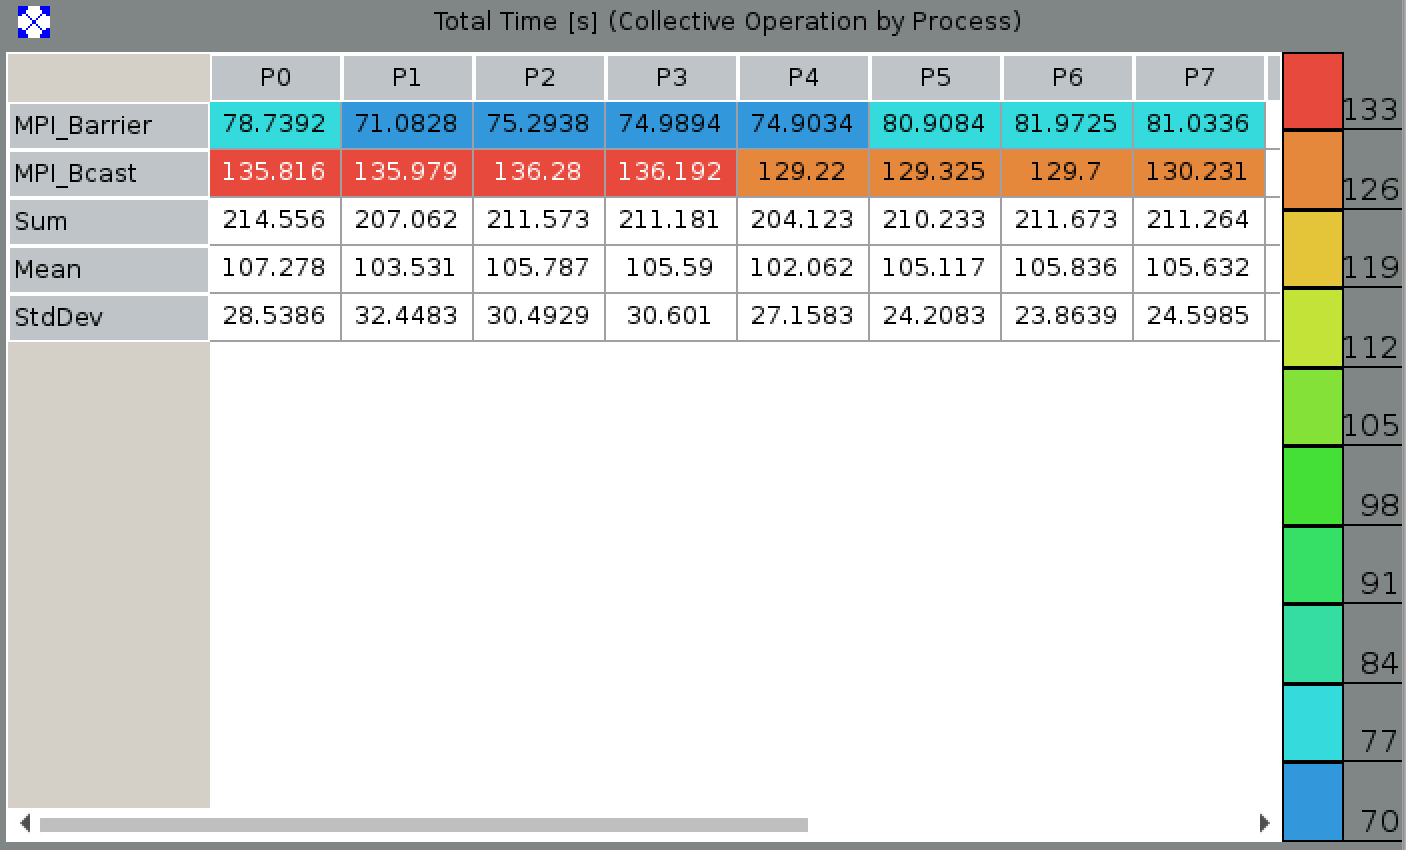
\includegraphics[width=0.8\textwidth]{figs/reductions}
\end{frame}

\begin{frame}[fragile]{Ways forward}
	\begin{itemize}[<+->]
		\item We found that:
		\begin{itemize}[<+->]
			\item \verb|MPI_Barrier| and \verb|MPI_Bcast| taking up a lot of time
			\item Communications are scattered throughout the program
			\item Very small amounts of compute between each communication
			\item Coordinator-worker pattern
			\item Some minor load balancing concerns
		\end{itemize}
		\item Things to think about
		\begin{itemize}[<+->]
			\item Can we use a peer-to-peer pattern instead?
			\item Can we increase the amount of work between communications?
			\item Is the direction we're parallelising appropriate?
		\end{itemize}
		\item If that fails, consider more advanced MPI features
	\end{itemize}
\end{frame}


\begin{frame}[fragile]{TIL \#1: MPI-IO}
	\begin{itemize}[<+->]
		\item Avoid channelling all I/O through a single rank/node
		\item Higher performance for reading and writing data
		\item Works really well with subarray types
	\end{itemize}\pause\small
	\begin{verbatim}
call MPI_File_Open(comm, 'con', MPI_Mode_Rdonly, &
MPI_Info_Null, mpi_fh)
call MPI_File_Set_View(mpi_fh, 0_8, MPI_Real, mpiio_type, &
"native", MPI_Info_Null)
call MPI_File_Read_All(mpi_fh, theta, &
3 * ksizex_l * ksizey_l * ksizet_l, &
MPI_Real, status)
call MPI_File_Close(mpi_fh)\end{verbatim}
\end{frame}

\begin{frame}[fragile]{Subarray types}
  \noindent\small
  	\begin{verbatim}
subroutine init_single_halo_type_4(direction, position, size4, datatype, typet)
  integer, intent(in) :: direction, position, size4
  type(MPI_Datatype), intent(in) :: datatype
  type(MPI_Datatype), intent(out) :: typet
  integer, dimension(4) :: sizes, subsizes, starts
  sizes = (/ ksizex_l + 2, ksizey_l + 2, ksizet_l + 2, size4 /)
  subsizes = (/ ksizex_l, ksizey_l, ksizet_l, size4 /)
  subsizes(direction+1) = 1
  starts = (/ 1, 1, 1, 0 /)
  starts(direction+1) = position
  call MPI_Type_Create_Subarray(4, sizes, subsizes, starts, &
                   MPI_Order_Fortran, datatype, typet)
  call MPI_Type_Commit(typet)
  return
end subroutine init_single_halo_type_4
\end{verbatim}	
\end{frame}


\begin{frame}[fragile]{Persistent MPI communications}
	\begin{itemize}[<+->]
		\item Each \verb|MPI_Send|/\verb|MPI_Recv| pair has an overhead
		\item For a tight loop, this wastes time
		\item Instead, use \verb|MPI_Send_Init|/\verb|MPI_Recv_Init| outside the loop
		\item \verb|MPI_Start|/\verb|MPI_StartAll| inside
		\item Also need \verb|MPI_Wait|/\verb|MPI_WaitAll|
		\item Speedup achieved will depend on architecture/communications fabric combination
		\item Collectives planned for MPI 3.2, e.g. \verb|MPI_AllReduce_Init|
	\end{itemize}
\end{frame}

\begin{frame}{Thanks for listening!}
	\Wider[0em]{\includegraphics[width=\textwidth]{figs/tsukuba-panorama}}
\end{frame}

\end{document}
